\documentclass[a4paper,10pt]{article}

\usepackage{amsmath}
\usepackage{amssymb}
\usepackage{graphicx}
\usepackage{subfigure}

\usepackage{geometry}
\geometry{left=2.5cm,right=2.5cm,top=2.5cm,bottom=2.5cm}

\usepackage{tikz}
\usetikzlibrary{arrows,shapes,chains}

\usepackage{float}

\usepackage{xcolor}

%opening
\title{December 2023, Summary on SPH Method}
\author{bcynuaa}
\date{\today}

\begin{document}

\maketitle
\tableofcontents

\section{Kernel Interpolation}

\subsection{Inspiration from $\delta$ Function}

\subsubsection{Dirac $\delta$ Function}

$\delta$ function is a function that is zero everywhere except at the origin, 
and its integral is 1. It is defined as
\begin{equation}
    \begin{aligned}
        \delta(x) = 
        \begin{cases}
            +\infty, & x = 0 \\
            0, & x \neq 0
        \end{cases}
        \quad \text{and} \quad
        \int_{-\infty}^{+\infty} \delta(x) \mathrm{d}x = 1
    \end{aligned}
\end{equation}

This function has a wide application in physics, 
especially in quantum mechanics. 
Such function has only math definition instead of detailed physical meaning.

$\delta$ function has 2 main properties:
\begin{itemize}
    \item $\delta(x) = 0, \forall x \neq 0$, which is called \textbf{locality} or \textbf{compact support}.
    \item $\int_{-\infty}^{+\infty} f(\xi) \delta(x - \xi)\mathrm{d}\xi = f(x)$, which is called \textbf{sifting property}.
\end{itemize}

These 2 properties are the key to the application of SPH method.

\begin{figure}[H]
    \centering
    \begin{tikzpicture}
        \draw[->] (-3, 0) -- (3, 0) node[right] {$x$};
        \draw[->] (0, -0.5) -- (0, 2) node[above] {$\delta(x)$};
        \draw[domain=-3:-0.1, samples=100] plot(\x, {0});
        \draw[domain=0.1:3, samples=100] plot(\x, {0});
        \draw[domain=-0.1:0.1, samples=100] plot(\x, {1.5});
        \draw (-0.1, 1.5) node[left] {$+\infty$};
    \end{tikzpicture}
    \caption{Dirac $\delta$ function}
    \label{fig:delta_function}
\end{figure}

In high-dimensional space, $\delta$ function is defined as
\begin{equation}
    \delta(\vec{r})=
    \begin{cases}
        +\infty, & \vec{r} = 0 \\
        0, & \vec{r} \neq 0
    \end{cases}
    \quad \text{and} \quad
    \int_{-\infty}^{+\infty} \delta(\vec{r}) \mathrm{d}\vec{r} = 1
\end{equation}
also, the sifting property is
\begin{equation}
    \int_{-\infty}^{+\infty} f(\vec{r}^\prime) \delta(\vec{r} - \vec{r}^\prime)\mathrm{d}\vec{r}^\prime = f(\vec{r})
\end{equation}

An inspiration comes out from the properties, 
which proposes the idea of using a $\delta$-like function to interpolate the physical quantities.

\subsubsection{$\delta$-like Function}

$\delta$-like function is a function that is zero everywhere except a small region around the origin,
and its integral is 1. It is defined as:
\begin{equation}
    \begin{aligned}
        W(x,h) = 
        \begin{cases}
            f(x), & |x| \leq h \\
            0, & |x| > h
        \end{cases}
        \quad \text{and} \quad
        \int_{-\infty}^{+\infty} W(x,h) \mathrm{d}x = 1
    \end{aligned}
\end{equation}
in high dimensional space, $W(\vec{r},h)$ is defined as
\begin{equation}
    \begin{aligned}
        W(\vec{r},h) = 
        \begin{cases}
            f(\vec{r}), & |\vec{r}| \leq h \\
            0, & |\vec{r}| > h
        \end{cases}
        \quad \text{and} \quad
        \int_{-\infty}^{+\infty} W(\vec{r},h) \mathrm{d}\vec{r} = 1
    \end{aligned}
\end{equation}

Here, $h$ is called \textbf{smoothing kernel length}. 
Also it's written as $h$, 
a radius ratio $t$ is often introduced to represent the kernel length $t h$ in application.
$t$ is called \textbf{smoothing kernel ratio}.
In equation formula, we use $h$ to represent the smoothing kernel length for simplicity.

A simple $\delta$-like function is the Gaussian function (1D):
\begin{equation}
    W(x,h) = \frac{1}{\sqrt{2\pi}h} \exp\left(-\frac{x^2}{2h^2}\right)
\end{equation}

\begin{figure}[H]
    \centering
    \begin{tikzpicture}
        \draw[->] (-3, 0) -- (3, 0) node[right] {$x$};
        \draw[->] (0, -0.5) -- (0, 3) node[above] {$W(x,h)$};
        \draw[domain=-3:-0.1, samples=100] plot(\x, {0});
        \draw[domain=0.1:3, samples=100] plot(\x, {0});
        \draw[domain=-0.1:0.1, samples=100] plot(\x, {1.5});
        \draw[domain=-3:3, samples=100] plot(\x, {exp(-(\x*\x)/0.2)/sqrt(2*pi)/0.2});
    \end{tikzpicture}
    \caption{$\delta$-like function: Gaussian function}
    \label{fig:delta_like_function_gaussian}
\end{figure}

$\delta$ function can be seen as a limit of Gaussian function when $h \rightarrow 0$:
\begin{equation}
    \lim_{h \rightarrow 0} W(x,h) = \delta(x)
\end{equation}

Although $\delta$-like function is not a real $\delta$ function, 
in numerical respect, 
it shares the same properties with $\delta$ function and can be used to interpolate the physical quantities.

\subsubsection{Let $\delta$-like Function Share Properties with $\delta$ Function}

$\delta$-like function shares the same properties with $\delta$ function:
\begin{itemize}
    \item $W(x,h) = 0, \forall |x| > h$, which is called \textbf{locality} or \textbf{compact support}.
    \item $\int_{-\infty}^{+\infty} f(\xi) W(x - \xi,h)\mathrm{d}\xi = f(x)$, which is called \textbf{sifting property}.
    \item $\int_{-\infty}^{+\infty} W(x,h) \mathrm{d}x = 1$, which is called \textbf{normalization}.
\end{itemize}

In $d$-dimensional space, 
$W(\vec{r},h)$ is zero everywhere except a $d$-dimensional sphere with radius $h$ around the origin.
With sifting property, 
$f(\vec{r})$'s value can be interpolated by $f(\vec{r}^\prime)$ distributed in a sphere with radius $h$ around $\vec{r}$.

\subsection{Kernel Function}

\subsubsection{Definition of Kernel Function}

Kernel function is a function that is zero everywhere except a small region around the origin,
and its integral is 1. It is defined as:
\begin{equation}
    \begin{aligned}
        W(\vec{r},h) = 
        \begin{cases}
            f(\vec{r}), & |\vec{r}| \leq h \\
            0, & |\vec{r}| > h
        \end{cases}
        \quad \text{and} \quad
        \int_{-\infty}^{+\infty} W(\vec{r},h) \mathrm{d}\vec{r} = 1
    \end{aligned}
\end{equation}

Here, $h$ is called \textbf{smoothing kernel length}.
It is an even function, as long as $|\vec{r}_1| = |\vec{r}_2|$, 
we have:
\begin{equation}
    W(\vec{r}_1, h) = W(\vec{r}_2, h)
\end{equation}

Usually, $W(\vec{r},h)$ is given by form of:
\begin{equation}
    W(\vec{r},h) = W(q) = W\left(\frac{r}{h}\right)\quad 
    r = |\vec{r}| = \sqrt{\vec{r}\cdot\vec{r}}=\sqrt{\sum_j x_j^2}
\end{equation}

\subsubsection{Derivation of Kernel Function}

Let's consider kernel function's derivation in $x_j$ direction:
\begin{equation}
    \begin{aligned}
        \frac{\partial W}{\partial x_j}&=
        \frac{\partial W}{\partial q}\frac{\partial q}{\partial r}\frac{\partial r}{\partial x_j}\\
        &=W^\prime \frac{1}{h}\frac{x_j}{r}
    \end{aligned}
\end{equation}

Thus $\nabla W$ is:
\begin{equation}
    \nabla W = \frac{1}{h} W^\prime \frac{\vec{r}}{r}
    = \frac{1}{h} W^\prime \hat{\vec{r}}
\end{equation}
$\hat{\vec{r}}$ is the unit vector of $\vec{r}$.

$\nabla W$ has the same direction with $\vec{r}$, and:
\begin{equation}
    \vec{r}\cdot \nabla W = \frac{r}{h} W^\prime\quad
    |\nabla W| = \left|\frac{1}{h} W^\prime\right|
\end{equation}
it's worth noting that $\nabla{W}$ will meet a singularity when $\vec{r}=\vec{0}$.

\subsection{Kernel Interpolation}

\subsubsection{Physical Quantity Kernel Interpolation}

As is discussed above, 
$\delta$-like function can be used to interpolate the physical quantities.
The interpolation formula is:
\begin{equation}
    f(\vec{r}) = \int_{-\infty}^{+\infty} f(\vec{r}^\prime) W(\vec{r} - \vec{r}^\prime,h)\mathrm{d}\vec{r}^\prime
\end{equation}

Now, let's consider the space domain discretized into particles, 
each particle is a material point with mass $m_i$ and position $\vec{r}_i$.

\begin{figure}[H]
    \centering
    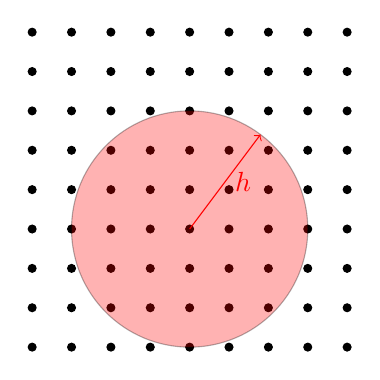
\begin{tikzpicture}
        \foreach \x in {0, 1, 2, 3, 4, 5, 6, 7, 8}
            \foreach \y in {0, 1, 2, 3, 4, 5, 6, 7, 8}
                \filldraw (0.5*\x, 0.5*\y) circle (0.05);
        \filldraw[fill=red, opacity=0.3] (0.5*4, 0.5*3) circle (1.5);
        \draw[->, red] (0.5*4, 0.5*3) -- (0.5*4+0.9, 0.5*3+1.2);
        \node[red] at (0.5*4+0.68, 0.5*3+0.6) {$h$};
    \end{tikzpicture}
\end{figure}

These particles have a scalar physical quantity $A_i$ and a vector physical quantity $\vec{v}_i$.
In SPH method, there values on particle $i$ can be interpolated with help of kernel function by 
particles $j$ near particle $i$:
\begin{equation}
    \begin{aligned}
        A_i &= \sum_j A_j W(\vec{r}_i - \vec{r}_j, h) \Delta V_j \\
        \vec{v}_i &= \sum_j \vec{v}_j W(\vec{r}_i - \vec{r}_j, h) \Delta V_j
    \end{aligned}
\end{equation}
$\Delta V_j$ is the volume of particle $j$, and $|\vec{r}_i - \vec{r}_j| \leq h$. 
As particle $j$'s mass $m_j$ and density $\rho_j$ are known, volume $\Delta V_j$ is substituted as below:
\begin{equation}
    \begin{aligned}
        A_i &= \sum_j \frac{m_j}{\rho_j} A_j W(\vec{r}_i - \vec{r}_j, h) \\
        \vec{v}_i &= \sum_j \frac{m_j}{\rho_j} \vec{v}_j W(\vec{r}_i - \vec{r}_j, h)
    \end{aligned}
\end{equation}

For simplicity, 
denote $W(\vec{r}_i - \vec{r}_j, h)$ as $W_{ij}$ as the kernel function is specified by $h$.
\begin{equation}
    \begin{aligned}
        A_i &= \sum_j \frac{m_j}{\rho_j} A_j W_{ij} \\
        \vec{v}_i &= \sum_j \frac{m_j}{\rho_j} \vec{v}_j W_{ij}
    \end{aligned}
\end{equation}

\subsubsection{Derivation of Kernel Interpolation}

The derivation of kernel interpolation is based on the sifting property of $\delta$-like function.
Let's consider a scalar's gradient value first:

\begin{equation}
    \begin{aligned}
        \nabla A(\vec{r}) &= 
        \int_{\Omega} \nabla A(\vec{r}^\prime) W(\vec{r} - \vec{r}^\prime,h)\mathrm{d}\vec{r}^\prime \\
        &\mathop{=}^{\text{symmetry}}
        \int_{\Omega} \nabla A(\vec{r}^\prime) W(\vec{r}^\prime-\vec{r},h)\mathrm{d}\vec{r}^\prime\\
        &\mathop{=}^{\text{Green's theorem}}
        \int_{\partial\Omega} A(\vec{r}^\prime) \vec{n} W(\vec{r}^\prime-\vec{r},h)\mathrm{d}\vec{r}^\prime
        - \int_{\Omega} A(\vec{r}^\prime) \nabla W(\vec{r}^\prime-\vec{r},h)\mathrm{d}\vec{r}^\prime\\
        &\mathop{=}^{\text{compact support}}
        - \int_{\Omega} A(\vec{r}^\prime) \nabla W(\vec{r}^\prime-\vec{r},h)\mathrm{d}\vec{r}^\prime\\
        &\mathop{=}^{\text{anti-symmetry}}
        \int_{\Omega} A(\vec{r}) \nabla W(\vec{r}-\vec{r}^\prime,h)\mathrm{d}\vec{r}^\prime\\
    \end{aligned}
\end{equation}

In the derivation, 
$\Omega$ is the space domain of the scalar $A(\vec{r})$, 
$\partial\Omega$ is the boundary of $\Omega$. 
For compact support, 
boundary part integral is zero.
In discretized form, 
such integral can be written as:
\begin{equation}
    \nabla A_i = \sum_j \frac{m_j}{\rho_j} A_j \nabla W(\vec{r}_i - \vec{r}_j, h)
\end{equation}

$\nabla W(\vec{r}_i - \vec{r}_j, h) = -\nabla W(\vec{r}_j - \vec{r}_i, h)$ for symmetry. 
In other people's papers and book, they usually denote $\nabla W(\vec{r}_i - \vec{r}_j, h)$ as $\nabla_i W_{ij}$. 
Here, we use $\nabla W_{ij}$ for simplicity:
\begin{equation}
    \nabla A_i = \sum_j \frac{m_j}{\rho_j} A_j \nabla W_{ij}
\end{equation}

However, this form of gradient is not that accurate. 
Now we consider a more accurate form of gradient. 
Multiply a scalar $\phi$ to the gradient:
\begin{equation}
    \phi\nabla A = \nabla(\phi A) - A\nabla\phi
\end{equation}

Let $\phi = \frac{1}{\rho}$, 
then:
\begin{equation}
    \begin{aligned}
        \frac{1}{\rho}\nabla A &= \nabla\left(\frac{A}{\rho}\right) - A\nabla\left(\frac{1}{\rho}\right)\\
        &=
        \nabla\left(\frac{A}{\rho}\right) + A\frac{\nabla\rho}{\rho^2}
    \end{aligned}
\end{equation}

In particle discretized form, we will have an approximation of $\frac{\nabla p}{\rho}$:
\begin{equation}
    \left(\frac{1}{\rho}\nabla A\right)_i
    =
    \sum_j m_j
    \left(
        \frac{A_j}{\rho_j^2}
        +
        \frac{A_i}{\rho_i^2}
    \right)\nabla W_{ij}
\end{equation}

What is worth noting
is that the choice of $\phi$ is not unique, 
different choice of $\phi$ will lead to different form of particle-discretized gradient.

For vector physical quantity $\vec{v}$,
we focus on the divergence of $\vec{v}$ and laplacian of $\vec{v}$.

\begin{equation}
    \begin{aligned}
        \nabla\cdot \vec{v} &=
        \int_{\Omega} \nabla\cdot \vec{v}(\vec{r}^\prime) W(\vec{r} - \vec{r}^\prime,h)\mathrm{d}\vec{r}^\prime \\
        &\mathop{=}^{\text{symmetry}}
        \int_{\Omega} \nabla\cdot \vec{v}(\vec{r}^\prime) W(\vec{r}^\prime-\vec{r},h)\mathrm{d}\vec{r}^\prime\\
        &\mathop{=}^{\text{Green's theorem}}
        \int_{\partial\Omega} \vec{v}(\vec{r}^\prime) \cdot \vec{n} W(\vec{r}^\prime-\vec{r},h)\mathrm{d}\vec{r}^\prime
        - \int_{\Omega} \vec{v}(\vec{r}^\prime) \cdot \nabla W(\vec{r}^\prime-\vec{r},h)\mathrm{d}\vec{r}^\prime\\
        &\mathop{=}^{\text{compact support}}
        - \int_{\Omega} \vec{v}(\vec{r}^\prime) \cdot \nabla W(\vec{r}^\prime-\vec{r},h)\mathrm{d}\vec{r}^\prime\\
        &\mathop{=}^{\text{anti-symmetry}}
        \int_{\Omega} \vec{v}(\vec{r}) \cdot \nabla W(\vec{r}-\vec{r}^\prime,h)\mathrm{d}\vec{r}^\prime\\
    \end{aligned}
\end{equation}

In discretized form:
\begin{equation}
    \nabla\cdot \vec{v}_i = \sum_j \frac{m_j}{\rho_j} \vec{v}_j \cdot \nabla W_{ij}
\end{equation}

It's the same problem that inaccuracy still exists in divergence of $\vec{v}$, 
thus we consider a more accurate form.
Multiply a scalar $\phi$ to the divergence:
\begin{equation}
    \phi\nabla\cdot \vec{v} = \nabla\cdot(\phi \vec{v}) - \vec{v}\cdot\nabla\phi
\end{equation}

Let $\phi = \rho$, 
then:
\begin{equation}
    \begin{aligned}
        \rho\nabla\cdot \vec{v} &= \nabla\cdot(\rho \vec{v}) - \vec{v}\cdot\nabla\rho\\
        &=
        \nabla\cdot(\rho \vec{v}) - \vec{v}\cdot\nabla\rho
    \end{aligned}
\end{equation}

In particle discretized form, we will have an approximation of $\rho\nabla\cdot \vec{v}$:
\begin{equation}
    \left(\rho\nabla\cdot \vec{v}\right)_i
    =
    \sum_j m_j
    (\vec{v}_j - \vec{v}_i)\cdot\nabla W_{ij}
    =-\sum_j m_j \vec{v}_{ij}\cdot\nabla W_{ij}
\end{equation}

$\vec{v}_{ij} = \vec{v}_i - \vec{v}_j$ is the velocity difference between particle $i$ and $j$.
For laplacian of $\vec{v}$,
the formula is much more complicated, 
of which the form will be given by detailed description in SPH method section.

\subsection{Frequently-used Kernel Functions}

\subsubsection{Cubic Spline Kernel Function}

Cubic spline kernel function is a piecewise function,
which is defined as:
\begin{equation}
    W(q)=\sigma_3
    \begin{cases}
        \begin{aligned}
            1-\frac{3}{2}q^2\left(1-\frac{q}{2}\right)\quad &0\leq q \leq 1 \\
            \frac{1}{4}(2-q)^3\quad &1\leq q \leq 2 \\
            0\quad &q > 2
        \end{aligned}
    \end{cases}\quad
    \sigma_3=
    \begin{cases}
        \begin{aligned}
            \frac{2}{3h} \quad &d=1 \\
            \frac{10}{7\pi h^2} \quad &d=2 \\
            \frac{1}{\pi h^3} \quad &d=3
        \end{aligned}
    \end{cases}
\end{equation}

\subsubsection{Gaussian Kernel Function}

Gaussian kernel function is a $\delta$-like function,
which is defined as:
\begin{equation}
    W(q)=
    \begin{cases}
        \begin{aligned}
            \sigma_g e^{-q^2}\quad &q \geq 0 \\
            0\quad &q < 0
        \end{aligned}
    \end{cases}\quad
    \sigma_g=
    \begin{cases}
        \begin{aligned}
            \frac{1}{\pi^{1/2}h} \quad &d=1 \\
            \frac{1}{\pi h^2} \quad &d=2 \\
            \frac{1}{\pi^{3/2} h^3} \quad &d=3
        \end{aligned}
    \end{cases}
\end{equation}

\subsubsection{Wendland Kernel Function}

Wendland kernel function is a $\delta$-like function, 
for WendlandC2 kernel function:
\begin{equation}
    W(q)=\alpha_d
    \begin{cases}
        \begin{aligned}
            \left(1-\frac{q}{2}\right)^4(2q+1)\quad &0\leq q \leq 2 \\
            0\quad &q > 2
        \end{aligned}
    \end{cases}\quad
    \alpha_d=
    \begin{cases}
        \begin{aligned}
            \frac{7}{4\pi h^2} \quad &d=2 \\
            \frac{21}{16\pi h^3} \quad &d=3
        \end{aligned}
    \end{cases}
\end{equation}

Another Wendland kernel function is WendlandC4 kernel function:
\begin{equation}
    W(q)=\alpha_d
    \begin{cases}
        \begin{aligned}
            \left(1-\frac{q}{2}\right)^6
            \left(\frac{35}{12}q^2+3q+1\right)\quad &0\leq q \leq 2 \\
            0\quad &q > 2
        \end{aligned}
    \end{cases}\quad
    \alpha_d=
    \begin{cases}
        \begin{aligned}
            \frac{9}{4\pi h^2} \quad &d=2 \\
            \frac{495}{256\pi h^3} \quad &d=3
        \end{aligned}
    \end{cases}
\end{equation}

\subsection{Reflection on Kernel Interpolation: Reduced to Traditional FDM}

As a new researcher to SPH method, 
the biggest question in my mind is that 
why the kernel interpolation can accurately interpolate the physical quantities. 
Kernel interpolation is more like a mathematical trick, rather than a numerical tool.

However, after coding and testing a simple SPH demo, 
I began to understand that kernel interpolation actually provide a cheap way to calculate a 
particle's contribution to scalar physical quantity and gradient around its neighbourhood.

Let's consider a particle $i$ in 1-D space, and a kernel function as below.

\begin{figure}[H]
    \centering
    \begin{tikzpicture}
        \draw[-] (-1,0)--(0,5)--(1,0);
        \draw[->] (-4,0)--(4,0) node[right] {$x$};
        \draw[->] (0,-0.5)--(0,6) node[above] {$W(x,h)$};
        \node at (1,-0.2) {$+h$};
        \node at (-1,-0.2) {$-h$};

        \node at (0.2, 5) {$u_i$};
        \node at (1.2, 5) {$u_{i+1}$};
        \node at (-0.8, 5) {$u_{i-1}$};

        \draw[dashed] (0,0)--(1,5)--(2,0);
        \draw[dashed] (0,0)--(-1,5)--(-2,0);
    \end{tikzpicture}
\end{figure}

\begin{equation}
    W(x,h)=
    \begin{cases}
        \begin{aligned}
            &-\frac{|x|}{h^2}+\frac{1}{h}\quad |x| \leq h \\
            &0 \quad |x| > h
        \end{aligned}
    \end{cases}
    \quad h \ll 1
\end{equation}

$W(x,h)$'s integral is 1:
\begin{equation}
    \int_{-h}^{+h} \left(-\frac{|x|}{h^2}+\frac{1}{h}\right)\mathrm{d}x = 1
\end{equation}

Particles of $i-1$, $i$ and $i+1$, has linear density $\rho_0$ and mass 
$m_j = \rho_0 h, j=i-1,i,i+1$.
\begin{equation}
    W(0,h)\frac{m_i}{\rho_0} = 1
\end{equation}

When $i$ particle and $j(=i+1)$ particle has a distance $h$, 
the interpolation will reduced to:
\begin{equation}
    \begin{aligned}
        u(x) = \left(1-\frac{x}{h}\right)u_i + \frac{x}{h}u_{i+1}\quad 
        0\leq x \leq h
    \end{aligned}
\end{equation}

And the gradient of $u(x)$ is:
\begin{equation}
    \begin{aligned}
        \frac{\partial u}{\partial x} = \frac{u_{i+1}-u_i}{h}
        =
        \partial_x W_i\frac{m_i}{\rho_0} u_i + \partial_x W_{i+1}\frac{m_{i+1}}{\rho_0} u_{i+1}
    \end{aligned}
\end{equation}

It seems that SPH method is reduced to a simple linear interpolation like finite difference method.

As 2 particles' relative distance changes, 
such kind of linear kernel function will cause trouble. 
It only works when the distacne is $h$. 
Thus
a more complicated kernel function is needed to fit for different distance.
That's the reason why kernel function can approximate the physical quantities and gradient.
\section{SPH Equation}

\subsection{Euler Discription and Lagrangian Discription in Continuum Mechanics}

Contrary to traditional CFD method, 
SPH is proposed based on Lagrangian discription in continuum mechanics.
In Lagrangian discription, 
the motion of a fluid particle is described by its position $\vec{x}$ and velocity $\vec{u}$.

Let's consider a physical quantity $\phi$ in a fluid particle. 
In Euler discription, 
the variation of $\phi$ is described by:
\begin{equation}
    \begin{aligned}
        \mathrm{d} \phi &= \frac{\partial \phi}{\partial t} \mathrm{d} t + \frac{\partial \phi}{\partial x} \mathrm{d} x + \frac{\partial \phi}{\partial y} \mathrm{d} y + \frac{\partial \phi}{\partial z} \mathrm{d} z\\
        &=
        \frac{\partial \phi}{\partial t} \mathrm{d} t +
        \left(
        \frac{\partial \phi}{\partial x} \frac{\mathrm{d} x}{\mathrm{d} t} +
        \frac{\partial \phi}{\partial y} \frac{\mathrm{d} y}{\mathrm{d} t} +
        \frac{\partial \phi}{\partial z} \frac{\mathrm{d} z}{\mathrm{d} t}
        \right) \mathrm{d} t\\
        &\rightarrow\\
        \frac{\mathrm{d} \phi}{\mathrm{d} t} &=
        \frac{\partial \phi}{\partial t} +
        u \frac{\partial \phi}{\partial x} +
        v \frac{\partial \phi}{\partial y} +
        w \frac{\partial \phi}{\partial z}
    \end{aligned}
\end{equation}

\begin{figure}[H]
    \centering
    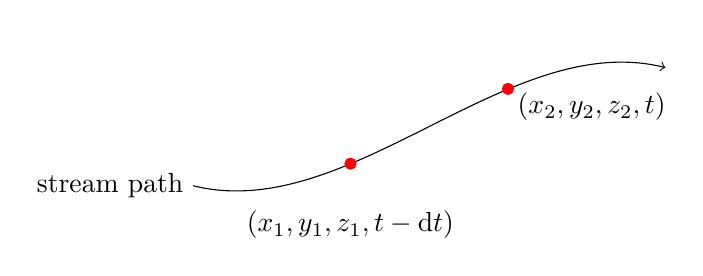
\begin{tikzpicture}
        \draw[->] (0,1) .. controls (2,0.5) and (4,3) .. (6,2.5);
        \node at (0,1) [left] {stream path};
        \node at (2, 0.5) {$(x_1,y_1,z_1,t-\mathrm{d}t)$};
        \filldraw[red] (2,1.28) circle (2pt);
        \filldraw[red] (4,2.23) circle (2pt);
        \node at (4,2) [right] {$(x_2,y_2,z_2,t)$};
    \end{tikzpicture}
\end{figure}

Here's a stream line where a fluid particle moves along. 
The particle's position is $(x_1,y_1,z_1,t-\mathrm{d}t)$ at time $t-\mathrm{d}t$ and $(x_2,y_2,z_2,t)$ at time $t$. 
For $\mathrm{d} t$ is small enough, 
$(x_1,y_1,z_1)$ and $(x_2,y_2,z_2)$ are very close to each other:
\begin{equation}
    (x_2-x_1, y_2-y_1, z_2-z_1) = (u\mathrm{d}t, v\mathrm{d}t, w\mathrm{d}t)
\end{equation}

When ths particle captures a physical quantity $\phi$, 
the variation of $\phi$ at position $(x_2,y_2,z_2)$ is (regardless the variation of $\phi$ in time):
\begin{equation}
    \mathrm{d}\phi = \phi(t) - \phi(t-\mathrm{d}t) = \frac{\partial \phi}{\partial x} u \mathrm{d}t + \frac{\partial \phi}{\partial y} v \mathrm{d}t + \frac{\partial \phi}{\partial z} w \mathrm{d}t
\end{equation}
the equation above declares that the variation of $\phi$ is caused by 
upstream physical quantity $\phi$. 
A time variation of $\phi$ is added as $\frac{\partial \phi}{\partial t}$ in unsteady flow field.

In Lagrangian discription, 
we track the motion of a fluid particle. 
Thus the part $\vec{u}\cdot\nabla\phi$ in the equation above is eliminated. 
Only fixed point in space will feel the change along the direction of flow field.
Thus the equation above is simplified as:
\begin{equation}
    \frac{\mathrm{d} \phi}{\mathrm{d} t} = \frac{\partial \phi}{\partial t}
\end{equation}

We use $\mathrm{D}^L$ and $\mathrm{D}^E$ to represent the variation of $\phi$ in Lagrangian discription and Euler discription respectively:
\begin{equation}
    \begin{aligned}
        \frac{\mathrm{D}^L \phi}{\mathrm{D} t} &= \frac{\partial \phi}{\partial t}\\
        \frac{\mathrm{D}^E \phi}{\mathrm{D} t} &= \frac{\partial \phi}{\partial t} + \vec{u}\cdot\nabla\phi
    \end{aligned}
\end{equation}

\subsection{Fluid Equation in Lagrangian Discription}

\subsubsection{Continuity Equation}

The continuity equation is derived from the conservation of mass. 
Considering a fluid particle with mass $m$ and volume $\delta V$, 
of which the shape is cuboid with $\Delta x$, $\Delta y$ and $\Delta z$ as its edges.
The volume can be represented as:
\begin{equation}
    \delta V = \Delta x \Delta y \Delta z
\end{equation}

\begin{figure}[H]
    \centering
    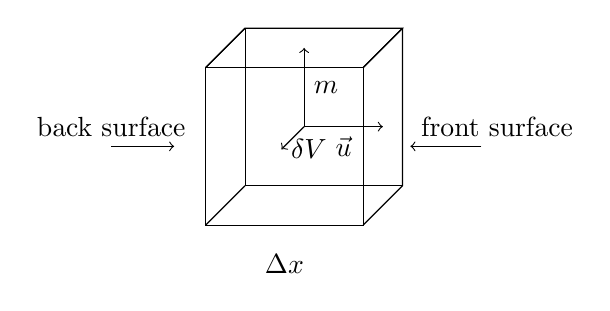
\begin{tikzpicture}
        % draw a cuboid with \delta x, \delta y and \delta z as its edges
        \draw (0,0) -- (0,2) -- (2,2) -- (2,0) -- cycle;
        \draw (0,2) -- (0.5,2.5) -- (2.5,2.5) -- (2,2);
        \draw (2,0) -- (2.5,0.5) -- (2.5,2.5);
        \draw (2.5,2.5) -- (2.5,0.5) -- (0.5,0.5);
        \draw (0.5,0.5) -- (0.5,2.5);
        \draw (0.5,0.5) -- (2.5,0.5);
        \draw (0,2) -- (0.5,2.5);
        \draw (2,2) -- (2.5,2.5);
        \draw (0,0) -- (0.5,0.5);
        % draw the velocity vector
        \draw[->] (1.25,1.25) -- (2.25,1.25);
        \node at (1.75,1.25) [below] {$\vec{u}$};
        % draw the mass vector
        \draw[->] (1.25,1.25) -- (1.25,2.25);
        \node at (1.25,1.75) [right] {$m$};
        % draw the volume vector
        \draw[->] (1.25,1.25) -- (1.25,1.25,0.75);
        \node at (1.25,1.25,0.75) [right] {$\delta V$};
        % front surface
        \node at (3.7,1) [above] {front surface};
        \draw[->] (3.5,1) -- (2.6,1);
        % back surface
        \node at (-1.2,1) [above] {back surface};
        \draw[->] (-1.2,1) -- (-0.4,1);
        % dx
        \node at (1,-0.5) {$\Delta x$};
    \end{tikzpicture}
\end{figure}

The mass of the fluid particle is:
\begin{equation}
    m = \rho \delta V = \rho \Delta x \Delta y \Delta z
\end{equation}

For conservation of mass, 
the variation of mass in the fluid particle is:
\begin{equation}
    \begin{aligned}
        0=\mathrm{d} m &= 
        \mathrm{d} (\rho \Delta x \Delta y \Delta z)\\
        &=
        \Delta x \Delta y \Delta z \mathrm{d} \rho +
        \rho \mathrm{d} (\Delta x \Delta y \Delta z)\\
    \end{aligned}
\end{equation}

In the cuboid model, as the back surface of cuboid moves with speed $u$, 
the front surface of cuboid moves with speed $u+\frac{\partial u}{\partial x}\Delta x$.
Thus the relative speed between the front surface and back surface is $\frac{\partial u}{\partial x}\Delta x$.
With a duration of $\mathrm{d} t$, 
the cuboid's length along $x$ direction will be changed from $\Delta x$ to:
\begin{equation}
    \Delta x\to 
    \Delta x + \frac{\partial u}{\partial x} \Delta x \mathrm{d} t
    = \Delta x (1 + \frac{\partial u}{\partial x} \mathrm{d} t)
\end{equation}
denote $\epsilon_i = \frac{\partial u_i}{\partial x_i}\mathrm{d} t$, 
we will have:
\begin{equation}
    \Delta x_i \to \Delta x_i (1+\epsilon_i)
\end{equation}
and the volume derivation during $\mathrm{d} t$ is:
\begin{equation}
    \begin{aligned}
        \mathrm{d} (\Delta x \Delta y \Delta z) &=
        \Delta x \Delta y \Delta z (1+\epsilon_x)(1+\epsilon_y)(1+\epsilon_z) - \Delta x \Delta y \Delta z\\
        &=
        \Delta x \Delta y \Delta z (\epsilon_x + \epsilon_y + \epsilon_z)\\
        &=
        \Delta x \Delta y \Delta z \nabla\cdot\vec{u} \mathrm{d} t
    \end{aligned}
\end{equation}
substitute the equation above into the equation of mass conservation:
\begin{equation}
    \delta V \mathrm{d}\rho + \rho \delta V \nabla \cdot \vec{u} \mathrm{d} t = 0
\end{equation}

Finally, we have the continuity equation in Lagrangian discription:
\begin{equation}
    \frac{\mathrm{D}^L \rho}{\mathrm{D} t} + \rho \nabla \cdot \vec{u} = 0
\end{equation}
which is usually written as:
\begin{equation}
    \frac{\partial \rho}{\partial t}=-\rho \nabla \cdot \vec{u}
\end{equation}

\subsubsection{Momentum Equation}

The momentum equation is derived from Newton's law.
Considering a fluid particle with mass $m$ and volume $\delta V$,
the external force acting on the fluid particle is $\vec{f}$:
\begin{equation}
    m\frac{\mathrm{D}^L \vec{u}}{\mathrm{D} t} = \vec{f}
\end{equation}

The external force $\vec{f}$ can be decomposed into two parts, 
one is the body force $\vec{f}_b$ and the other is the surface force $\vec{f}_s$:
\begin{equation}
    \vec{f} = \vec{f}_b + \vec{f}_s
\end{equation}

For body force, which is usually gravity, electric force, magnetic force, etc., 
the force is proportional to the mass of the fluid particle:
\begin{equation}
    \vec{f}_b = m \vec{g}
\end{equation}

Surface force is usually more complicated. 
Under Stokes assumption, 
the surface foce acting on $j$-th surface along direction $i$'s $\tau_{ij}$ is:
\begin{equation}
    \tau_{ij} = (-p + \lambda\nabla\cdot\vec{u})\delta_{ij} 
    + \mu\left(\frac{\partial u_i}{\partial x_j} + \frac{\partial u_j}{\partial x_i}\right)
\end{equation}
what's more, Stokes assumption requires that in steady flow field, 
the pressure force is equal to the surface force:
\begin{equation}
    \tau_{11}+\tau_{22}+\tau_{33} = -3p 
    + 3\lambda\nabla\cdot\vec{u} 
    + 2\mu \nabla \cdot \vec{u}
    \to
    \lambda = -\frac{2}{3}\mu
\end{equation}

Thus the surface force is:
\begin{equation}
    \vec{f}_s = \nabla\cdot [\tau]
    = 
    -\nabla p + \mu \nabla^2 \vec{u} + \frac{\mu}{3}\nabla(\nabla\cdot\vec{u})
\end{equation}
equation above requires that $\mu$ is constant in fluid field. 
Moreover, when we discuss a incompressible fluid, 
$\frac{\mu}{3}\nabla(\nabla\cdot\vec{u})$ is eliminated.

Finally, we have the momentum equation in Lagrangian discription:
\begin{equation}
    \frac{\mathrm{D}^L \vec{u}}{\mathrm{D} t} = - \frac{1}{\rho}\nabla p + \frac{\mu}{\rho}\nabla^2\vec{u} + \vec{g}
\end{equation}
which is usually written as:
\begin{equation}
    \frac{\partial \vec{u}}{\partial t} = - \frac{1}{\rho}\nabla p + \frac{\mu}{\rho}\nabla^2\vec{u} + \vec{g}
\end{equation}

\subsubsection{Energy Equation}

SPH method usually focus on motion of incompressible fluid like water, 
energy equation is not necessary in this case. 
I will finish this part later.

\subsubsection{Equation of State}

In SPH method, 
the equation of state is largely depend on the scheme. 
A large widely used scheme is weakly compressible scheme:
\begin{equation}
    \label{eq:Weakly Compressible Scheme}
    p = \frac{c_0^2\rho_0}{\gamma}
    \left[
        \left(\frac{\rho}{\rho_0}\right)^\gamma - 1
    \right]
\end{equation}
when $\rho-\rho_0$ is small enough, 
the equation above can be simplified as:
\begin{equation}
    \begin{aligned}
        p &= \frac{c_0^2\rho_0}{\gamma}
        \left[
            \left(1+\frac{\rho-\rho_0}{\rho_0}\right)^\gamma - 1
        \right]\\
        &\approx \frac{c_0^2\rho_0}{\gamma}
        \left[
            1 + \gamma\frac{\rho-\rho_0}{\rho_0} - 1
        \right]\\
        &= c_0^2 (\rho - \rho_0)
    \end{aligned}
\end{equation}

In SPHysics, and Monaghan's SPH method, $\gamma=7$ and $c_0$ is 
an artificial speed of sound, which is usually set to $10\max\{U_{\max},\sqrt{gL_{\max}}\}$.

\subsection{SPH Discretization}

\subsubsection{Spatial Discretization}

In this section, 
we only consider restrict formula of SPH discretization. 
Tricks like artificial viscosity, XSPH, kernel correction, etc. 
will be discussed in the next section.

As is discussed above, 
fluid equation in Lagrangian discription can be discretized as:
\begin{equation}
    \begin{aligned}
        \left(\frac{\partial\rho}{\partial t}\right)_i
        &=
        \sum_j m_j \vec{u}_{ij} \cdot \nabla W_{ij}\\
        \left(\frac{\partial\vec{u}}{\partial t}\right)_i
        &=
        -\sum_j m_j \left(\frac{p_i}{\rho_i^2} + \frac{p_j}{\rho_j^2}\right) \nabla W_{ij} + 
        \vec{g} + 
        \sum_j \frac{4m_j(\mu_i+\mu_j)\vec{r}_{ij}\cdot \nabla W_{ij}}{(\rho_i+\rho_j)^2[r_{ij}^2+(0.1h)^2]}\vec{u}_{ij}\\
        \left(\frac{\partial \vec{x}}{\partial t}\right)_i
        &=
        \vec{u}_i
    \end{aligned}
\end{equation}

\subsubsection{Time Discretization}

For each step needs a neighbour search over all particles.
Thus traditional Runge-Kutta method is not suitable for SPH method.

Current code uses explicit Euler method. 
Another widely used method is predictor-corrector method,
which will added in future work.

CFL number is used to control the time step.
A conservative time step is:
\begin{equation}
    \Delta t=\frac{h}{10c_0}
\end{equation}

As $U_{\max}$ is usually smaller than $0.1c_0$,
each time step only allows a particle to move a distance of $0.01h$ in this format.

\subsection{Boundary Condition}

\subsubsection{Compulsive Wall Boundary Condition}

Monaghan in his paper 'Solitary Waves on a Cretan Beach' first proposed the conpulsive boundary condition.
He aranged a series of fixed wall particles on the boundary of the fluid field 
which will have a compulsive force on the fluid particles.

\begin{figure}[H]
    \centering
    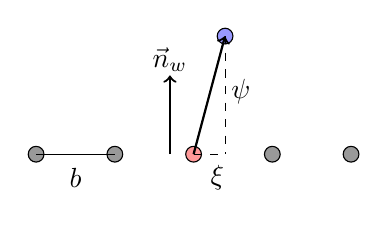
\begin{tikzpicture}
        \foreach \x in {0,1,3,4}
        \draw[fill=black!40!white, draw=black] (\x,0) circle (0.1);
        \draw[fill=blue!40!white, draw=black] (2.4,1.5) circle (0.1);
        \draw[fill=red!40!white, draw=black] (2,0) circle (0.1);
        
        \draw[->, thick] (2,0) -- (2.4,1.5);
        \draw[->, thick] (1.7,0) -- (1.7,1);
        \node at (1.7,1.2) {$\vec{n}_w$};
        \draw[dashed] (2.4,1.5) -- (2.4,0);
        \draw[dashed] (2, 0) -- (2.4,0);

        \draw[-] (0,0)--(1,0);
        \node at (0.5, -0.3) {$b$};

        \node at (2.6,0.8) {$\psi$};
        \node at (2.3, -0.3) {$\xi$};
    \end{tikzpicture}
\end{figure}

With wall particle's gap $b$ and normal vector $\vec{n}_w$, 
considering a fluid particle's position at $(\xi, \psi)$ relative to a wall particle, 
it will feel a compulsive force $\vec{f}_w$:
\begin{equation}
    \vec{f}_w=P(\psi)R(\xi)\epsilon(u_{\perp},z)\vec{n}_w
\end{equation}

$\psi$ is the distance between the fluid particle and the wall particle,
$\xi$ is the projection of the fluid particle on the wall particle.

The part $P(\psi)$ is the compulsive force caused by the distance between the fluid particle and the wall particle.
It is designed to be a function with singularity at $\psi=0$:
\begin{equation}
    P(\psi)=A\frac{1}{\sqrt{q}}(1-q)
\end{equation}
in which $A=\frac{1}{h}(0.1c_i)^2$ and $q=\frac{\psi}{2h}$.
$c_i$ is the artificial speed of sound in fluid particle $i$.
Although the equation is proved wrong in my personal practice, 
I will discuss it later.

The part $R(\xi)$ is the compulsive force caused by the projection of the fluid particle on the wall particle.
It is designed to be a periodic function:
\begin{equation}
    R(\xi)=\frac{1}{2}\left[
        1+\cos\left(\frac{2\pi\xi}{b}\right)
    \right]
\end{equation}

However, as I practice the compulsive boundary condition, still particles will 
penetrate the wall. I fix this problem by analysing the characteristic of cosine function.
\begin{figure}[H]
    \centering
    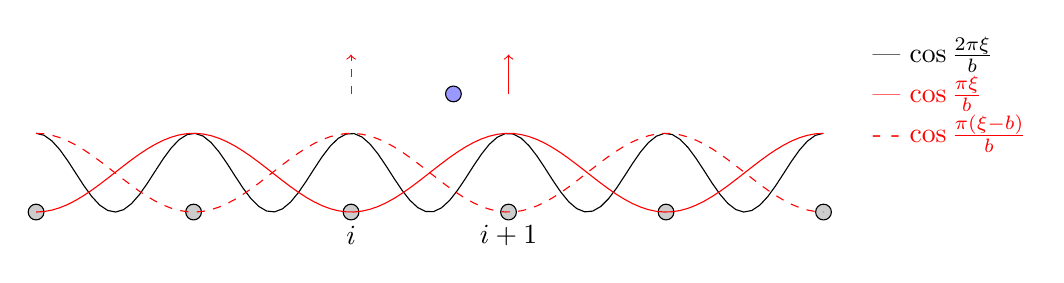
\begin{tikzpicture}
        \foreach \x in {-3,-2,-1,0,1,2}
        \filldraw[fill=gray!40!white, draw=black] (2*\x,0) circle (0.1);
        % plot cos 2pi x
        \draw[domain=-3:2,samples=100] plot (\x*2,{0.5+0.5*cos(360*\x)});
        % plot cos pi x
        \draw[domain=-3:2,samples=100,red] plot (\x*2,{0.5+0.5*cos(180*\x)});
        \draw[domain=-3:2,samples=100,red,dashed] plot (\x*2,{0.5+0.5*cos(180*(\x-1)});
        % fluid particle
        \filldraw[fill=blue!40!white, draw=black] (-0.7,1.5) circle (0.1);
        
        \draw[->,red] (0,1.5)--(0,2.0);
        \draw[->,red,dashed] (-2,1.5)--(-2,2.0);

        \node[right] at (4.5,2) {---  $\cos \frac{2\pi\xi}{b}$};
        \node[right,red] at (4.5,1.5) {---  $\cos \frac{\pi\xi}{b}$};
        \node[right,red] at (4.5,1) {- -  $\cos \frac{\pi(\xi-b)}{b}$};

        \node at (-2, -0.3) {$i$};
        \node at (0, -0.3) {$i+1$};
    \end{tikzpicture}
\end{figure}

As is shown in the figure above,
a fluid particle is influenced by 2 wall particles,
one is the wall particle at $\xi$ and the other is the wall particle at $b-\xi$.
\begin{equation}
    \begin{aligned}
        R_{i} &= \frac{1}{2}\left[
            1+\cos\left(\frac{\pi\xi}{b}\right)
        \right]\\
        R_{i+1} &= \frac{1}{2}\left[
            1+\cos\left(\frac{\pi(b-\xi)}{b}\right)
        \right]\\
        R_{i}+R_{i+1} &= 1+\frac{1}{2}\left[
            \cos\left(\frac{\pi\xi}{b}\right) + \cos\left(\frac{\pi(b-\xi)}{b}\right)
        \right]=1
    \end{aligned}
\end{equation}
this will garantee that a particle fly along the wall feels a constant compulsive force.
However, 
if use equation in SPHysics documnent and Delong Xu's book or Rogers's paper, 
the compulsive force will be:
\begin{equation}
    \begin{aligned}
        R_{i} &= \frac{1}{2}\left[
            1+\cos\left(\frac{2\pi\xi}{b}\right)
        \right]\\
        R_{i+1} &= \frac{1}{2}\left[
            1+\cos\left(\frac{2\pi(b-\xi)}{b}\right)
        \right]\\
        R_{i}+R_{i+1} &= 1+\frac{1}{2}\left[
            \cos\left(\frac{2\pi\xi}{b}\right) + \cos\left(\frac{2\pi(b-\xi)}{b}\right)
        \right]=1+\cos\left(\frac{2\pi\xi}{b}\right)
    \end{aligned}
\end{equation}

When $\xi=\frac{b}{2}$, $R_{i}+R_{i+1}=0$. 
When $\xi=0$, $R_{i}+R_{i+1}=2$, which is twice of the compulsive force at $\xi=\frac{b}{2}$.
This indicates that a fluid particle will penetrate the wall in the middle of two wall particles 
but will be pushed back when it is close to a wall particle.
After all, I modify this equation to:
\begin{equation}
    R(\xi)=\frac{1}{2}\left[
        1+\cos\left(\frac{\pi\xi}{b}\right)
    \right]
\end{equation}

A coefficient $\epsilon(u_{\perp},z)$ is added to the compulsive force to 
modify the compulsive force when the fluid particle is close to the wall.

\begin{equation}
    \epsilon(u_{\perp},z)=\epsilon (u_{\perp})+\epsilon(z)
\end{equation}
其中:
\begin{equation}
    \epsilon(u_{\perp})=
    \begin{cases}
        0 &\quad u_{\perp}\geq 0\\
        -\frac{20u_{\perp}}{c_0} &\quad -20u_{\perp}<c_0\\
        1 &\quad -20u_{\perp}\geq c_0
    \end{cases}
\end{equation}
\begin{equation}
    \epsilon(z)=
    \begin{cases}
        0 &\quad z\geq 0\\
        -\frac{z}{h_0} &\quad -h_0<z<0\\
        1 &\quad -h_0\geq z
    \end{cases}
\end{equation}
where $h_0$ is the depth of the location of the wall particle. 
$\epsilon(z)$ is a modification to pressure depth.
And $u_{\perp}$ is the velocity of the fluid particle along the normal vector of the wall particle.
$\epsilon(u_{\perp})$ is a modification to the velocity of the fluid particle along the normal vector of the wall particle.

In Monaghan's paper, 
$(0.1c_i)^2$ can be used as $\frac{|p|}{\rho}$, 
which is the pressure depth of the fluid particle. 
And the coefficient $\epsilon$ can be used in another form by Monaghan:
\begin{equation}
    A=\frac{1}{h}(0.01c^2 -\beta c\vec{u}_i\cdot\vec{n}_w)
\end{equation}
where:
\begin{equation}
    \beta=
    \begin{cases}
        \begin{aligned}
            0 &\quad \vec{u}_i\cdot\vec{n}_w\geq 0\\
            1 &\quad \vec{u}_i\cdot\vec{n}_w<0
        \end{aligned}
    \end{cases}
\end{equation}

\subsubsection{Open Boundary Condition}

Open boundary condition is widely applied in traditional CFD method.
However, 
SPH method will face difficulty when open boundary condition is applied for
there will be particles flying out of and flying into the fluid field.
This means that the fluid field's particle number is varying within time, 
which cause trouble in coding.

I will finish this in future work.

\subsubsection{Other Boundary Conditions}

Other boundary conditions.
\section{Tricks}

Although my tutor has told me that he doesn't care about the tricks and details, 
but code still runs on these tricks and details.
I will list some detailed tricks here, 
which is of great significnce to running program properly.

\subsection{The Direaction of $\nabla W_{ij}$ and Low Pressure Problem}

As mentioned above, $\nabla W_{ij}$ has the direction as $\vec{r}_i - \vec{r}_j$.
However, as $W^\prime(q)$ is below zero, 
thus actually $\nabla W_{ij}$ has the direction as $\vec{r}_j - \vec{r}_i$:

\begin{figure}[H]
    \centering
    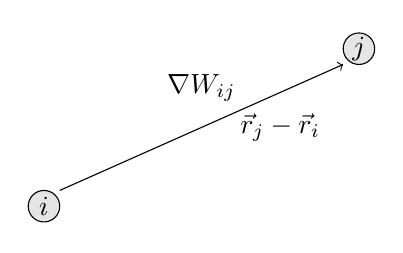
\begin{tikzpicture}
        \filldraw[fill=gray!20!white, draw=black] (0,0) circle (0.2);
        \filldraw[fill=gray!20!white, draw=black] (4,2) circle (0.2);

        \node at (0,0) {$i$};
        \node at (4,2) {$j$};

        \node at (3.0, 1) {$\vec{r}_j - \vec{r}_i$};
        % arrow without head
        \draw[->] (0.2,0.2)--(3.8,1.8);
        
        \node at (2, 1.5) {$\nabla W_{ij}$};
    \end{tikzpicture}
\end{figure}

Let's turn to the continuity equation in SPH method:
\begin{equation}
    \frac{d\rho_i}{dt} = \sum_j m_j \vec{u}_{ij} \cdot \nabla W_{ij}
\end{equation}
as long as 2 particles approach each other, 
$\vec{u}_{ij}\cdot \nabla W_{ij}$ will be positive, 
leading to an increase of $\rho_i$ and $\rho_j$.
You may see that the increase of density is symmetric to these 2 particles.

When eq.\ref{eq:Weakly Compressible Scheme} is introduced, 
a problem arises that particles captures lower density ($\rho<\rho_0\to$negative pressure) 
will get together from motion equation.
A group of particles approaching each other will cause a large increase on density 
as well as a sharp increase on pressure.
High pressure field will push these particles away from each other, 
and emit them out like a bullet.

\begin{figure}[H]
    \centering
    \subfigure[low pressure field in calculation]{
        \includegraphics[width=0.4\textwidth]{images/low_pressure_field.png}
    }
    \subfigure[emit particles out like bullets]{
        \includegraphics[width=0.48\textwidth]{images/emit_like_bullet.png}
    }
\end{figure}

It's worth noting that a ratio of smoothing length $h$ and particle's initial gap $\mathrm{d}r$ 
will influence the calculation result.
When $h/\mathrm{d}r$ is small, 
a particle is influenced by a few particles around it.
And the fluid will flow more loosely like 'ocean balls' in children's playground.
When $h/\mathrm{d}r$ is large, 
a particle is influenced by a lot of particles around it.
And the fluid will flow more tightly like 'water' in a glass.

Although for high numerical pricision, 
$h/\mathrm{d}r$ should be as large as possible, 
this may cause the low pressure problem leading to numerical instability.
In my personal practice,
I found that $h/\mathrm{d}r=3$ corresponds to reference's result, 
but will cause low pressure problem at the same time in standard case collapse onto dry bottom.

To conclude, 
we should avoid particles with low density getting together in weakly-compressible-state SPH method.
A possible way is to generate an artificial repulsive force between 2 particles 
added to pressure force part (inspired from Lenard-Jones repulsive force):
\begin{equation}
    \vec{f}_i^p = 
    -\sum_j 
    m_j 
    \left(
        \frac{p_i}{\rho_i^2} + \frac{p_j}{\rho_j^2} + R_{ij}
    \right)\nabla W_{ij}
\end{equation}
where $R_{ij}$ equals to ($\Delta p$ is the initial gap between 2 particles):
\begin{equation}
    R_{ij} = 
    0.01
    \left(
        \frac{p_i}{\rho_i^2} + \frac{p_j}{\rho_j^2}
    \right)
    \frac{W(r_{ij}, h)}{W(\Delta p, h)}
\end{equation}

\subsection{XSPH Method}

XSPH method was first proposed by Monaghan,
aiming at avoiding particles penetrating each other.
The main idea is to add a correction term to velocity when moving particles:
\begin{equation}
    \frac{\mathrm{d}\vec{r}_i}{\mathrm{d}t} = \vec{u}_i - \epsilon \sum_j m_j \frac{\vec{u}_{ij}}{\bar{\rho}_{ij}} W_{ij}
\end{equation}
where $\bar{\rho}_{ij} = \frac{1}{2}(\rho_i + \rho_j)$,
and $\epsilon$ varies from 0 to 1.
Monaghan suggested that $\epsilon$ should be set to $0.5$.

My tutor told me that XSPH method's parameter $\epsilon$ can be modified artificially.
At current stage, I have an initial idea that use a function to determine the 
disorder degree of particles.
The value of $\cos<\vec{u}_i, \vec{u}_j>$ can be used to measure the disorder degree of 2 particles.
When $\cos<\vec{u}_i, \vec{u}_j>$ is close to $1$, 
which means 2 particles are moving in the same direction, 
thus $\epsilon$ should be set to a small value.
When $\cos<\vec{u}_i, \vec{u}_j>$ is close to $-1$,
which means 2 particles are moving in the opposite direction,
thus $\epsilon$ should be set to a large value.

The XSPH method can be added to the SPH method easily and improves the stability,
but can't avoid low-pressure problem completely.

% red warning
\textcolor{red}{Warning, 2023.12.26:} I found that XSPH method in unsteady problem will lead to
unpredictable error when high-speed particles penetrate low-speed particles.

\subsection{Kernel Correction}

For particles close to boundary (like free surface boundary and wall boundary),
the kernel function will be cut off by boundary.
Thus a kernel correction should be applied to these particles.

\begin{figure}[H]
    \centering
    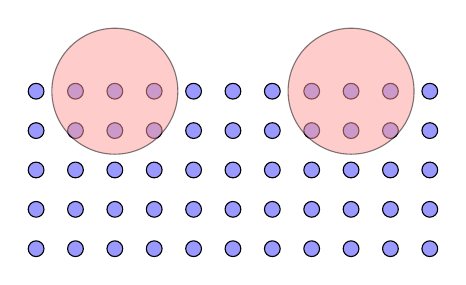
\begin{tikzpicture}
        % several particles
        % 4 row, 5 column
        \foreach \x in {0,1,2,3,4,5,6,7,8,9,10}
        \foreach \y in {0,1,2,3,4}
        \filldraw[fill=blue!40!white, draw=black] (0.5*\x,0.5*\y) circle (0.1);
        % draw a circle at the top row in the middle, alpha = 0.5
        \draw[fill=red!40!white, draw=black, opacity=0.5] (1.0,2) circle (0.8);
        % draw a circle at the top row in the middle, alpha = 0.5
        \draw[fill=red!40!white, draw=black, opacity=0.5] (4.0,2) circle (0.8);
    \end{tikzpicture}
\end{figure}
\begin{equation}
    \hat{\rho}_i = \frac{
        \sum_j m_j W_{ij}
    }{
        \sum_j \frac{m_j}{\rho_j}W_{ij}
    }
\end{equation}

For particles inside the fluid field,
kernel function which is a $\delta$-like function should gaurantee that:
\begin{equation}
    \sum_j \frac{m_j}{\rho_j} W_{ij} \approx 1
\end{equation}

This kind of kernel correction is fit for other physical quantities as well.
Any physical quantity $A$ can be corrected by:
\begin{equation}
    \hat{A}_i = \frac{
        \sum_j \frac{m_j}{\rho_j} A_j W_{ij}
    }{
        \sum_j \frac{m_j}{\rho_j} W_{ij}
    }
\end{equation}

Kernel correction is not necessary in each time step. 
A recommended time step interval is 30 time steps.
It's of great significnce to gaurantee calculation stability.

\subsection{Design of Compulsive Boundary Condition}

Compulsive boundary condition is applied by aranging a group of wall 
particles at the boundary.
As is mentioned above,
this compulsive boundary condition is designed by a singular function:
\begin{equation}
    f(q) = \frac{1}{\sqrt{q}}(1-q) \quad q=\frac{\psi}{2h}
\end{equation}

\begin{figure}[H]
    \centering
    \begin{tikzpicture}
        % plot f(q)
        \draw[->] (-0.5,0)--(1.5,0) node[right] {$q$};
        \draw[->] (0,-0.5)--(0,1.8) node[above] {$f(q)$};
        \draw[domain=0.1:1, samples=100] plot(\x, {0.5*1/sqrt(\x)*(1-\x)});
    \end{tikzpicture}
\end{figure}

This function will meet a sharp increase as $q$ approaches $0$ from $1$.
When a pair of fluid particle and wall particle is close enough at initial time,
the compulsive force will be very large and push the fluid particle away from the wall particle,
resulting in a non-physics result.
Although Monaghan proposed that $q=\psi/2\Delta p$ and papers citing his article 
proposed that $q=\psi/2h$.
No matter which one is used,
the main idea is to avoid initial gap between fluid particle and wall particle being smaller 
than the influence radius of $f(q)$.
\begin{figure}[H]
    \centering
    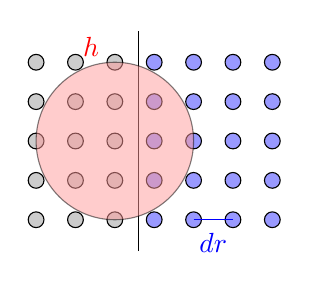
\begin{tikzpicture}
        % fluid particle
        \foreach \x in {0,1,2,3}
        \foreach \y in {0,1,2,3,4}
        \filldraw[fill=blue!40!white, draw=black] (0.5*\x,0.5*\y) circle (0.1);
        \draw[-] (-0.2,-0.4) -- (-0.2,2.4);
        % boundary particle
        \foreach \x in {-3,-2,-1}
        \foreach \y in {0,1,2,3,4}
        \filldraw[fill=gray!40!white, draw=black] (0.5*\x,0.5*\y) circle (0.1);
        
        \filldraw[fill=red!40!white, draw=black,opacity=0.5] (-0.5,0.5*2) circle (1.);

        \node[red] at (-0.8,2.2) {$h$};

        \draw[-,blue] (0.5,0) -- (1,0);
        \node[blue] at (0.75,-0.3) {$dr$};
    \end{tikzpicture}
\end{figure}

What's more, 
Monaghan said the detaild form of $f(q)$ is not important as long as 
$f(q)$ has the property of $f(0)=\infty$ and $f(1)=0$.
However, in my personal practice,
the coefficient is still important which determines the stiffness of compulsive boundary condition.
The fluid particle's splashing speed largely depend on this.

\subsection{Background Pressure}

In senior-high-school physics,
the atmospheric pressure is about $101325\mathrm{Pa}$.
This part is usually ignored in steady water field.

Here's always a problem I can't understand in SPH that:
\begin{equation}
    \phi\nabla p = \nabla (\phi p) - p\nabla \phi
\end{equation}

Apply $\nabla$'s operator with kernel interpolation method:
\begin{equation}
    \begin{aligned}
        \phi_i\nabla p_i
    &= \sum_j 
    \frac{m_j}{\rho_j} \phi_j p_j \nabla_i W_{ij}
    -\sum_j
    p_i\frac{m_j}{\rho_j} \phi_i \nabla W_{ij}\\
    \nabla p_i
    &=
    \frac{1}{\phi_i}\sum_j
    \frac{m_j}{\rho_j} \phi_j (p_j-p_i) \nabla W_{ij}
    \end{aligned}
\end{equation}
let $\phi=1$ we have:
\begin{equation}
    \nabla p_i
    =
    \sum_j
    \frac{m_j}{\rho_j} (p_j-p_i) \nabla W_{ij}
\end{equation}

This format of kernel interpolation is correct but not usually widely applied in 
SPH. Instead, the following format is widely used:
\begin{equation}
    \nabla p_i
    =\rho_i
    \sum_j m_j
    \left(
        \frac{p_i}{\rho_i^2} + \frac{p_j}{\rho_j^2}
    \right)\nabla W_{ij}
\end{equation}

When background is added into each particle's pressure,
the 2 kernel interpolation methods are quite different.
$p_j-p_i$ part neglects the background pressure, 
while $\frac{p_i}{\rho_i^2} + \frac{p_j}{\rho_j^2}$ scheme
will have an extra part $p_0\left(
    \frac{1}{\rho_i^2} + \frac{1}{\rho_j^2}
\right)$.

A possible reason is that SPH method
uses $\delta$-like function as kernel function, which actually
performs as a probability distribution like wave function in quantum mechanics.
This indicates that SPH method requires a large number of neighbour particles to
eliminate the influence of single one nearby particle.
Thus focus on 2 particles' interaction may not reflect the real physical phenomenon.
From perspective of probability,
SPH kernel interpolation method uses enough particles to approximate the real physical phenomenon,
just like Large Number Law.

With this in mind, 
a particle's front and back neighbour particles will 
balance the background pressure as to kernel interpolation on the particle itself.

Thus when background pressure is added, 
gas particles capturing with constant atmospheric pressure should be 
included into calculation, which is useless for water field simulation.

\subsection{$\delta^+$ SPH Model: A Kind of Density Filter and Stabilizer}

$\delta^+$ SPH model is adopted to avoid pressure oscillation.
For in SPH, pressure only depends on density, 
thus the stability of density field is of great significnce.

With this in mind, an additional part is added to continuity equation:
\begin{equation}
    \left(
        \frac{\partial \rho}{\partial t}
    \right)_i
    =
    \sum_j m_j \vec{u}_{ij} \cdot \nabla W_{ij}
    +
    h c_0 \delta
    \sum_j  \frac{m_j}{\rho_j} \vec{D}_{ij}\cdot \nabla W_{ij}
\end{equation}
$\vec{D}_{ij}$'s part is complicated. We first propose a concept of re-normalization matrix 
$[L]_i$ as below (tensor multiply instead of dot contraction):
\begin{equation}
    [L]_i = \left[\sum_j \frac{m_j}{\rho_j}\vec{r}_{ij}\nabla W_{ij}\right]^{-1}
\end{equation}
$[L]_i$ has the size of $d\times d$ where $d$ is the dimension of space.
And its uinit is $m^{-1}$.

The matrix is a kind of local gradient operator matrix, 
where the re-normalized gradient of density $\nabla \rho_i^L$ can be calculated by:
\begin{equation}
    \nabla \rho_i^L = \sum_j \frac{m_j}{\rho_j}\rho_{ij}
    [L]_i \cdot \nabla W_{ij}
\end{equation}

Finally, $\vec{D}_{ij}$ is given by:
\begin{equation}
    \vec{D}_{ij} = 
    \left[
        2\rho_{ij} - 
        \left(
            \nabla \rho_i^L + \nabla \rho_j^L
        \right)\cdot \vec{r}_{ij}
    \right]
    \frac{\vec{r}_{ij}}{r_{ij}^2 + 0.01h^2}
\end{equation}

$\delta$ is a dimensionless parameter, 
which is usually set to $0.1$.
As described in Monaghan's paper,
$\delta^+$ SPH model is a kind of density filter and stabilizer,
which can even lead to better results than ICSPH in WCSPH method.

% warning
\textcolor{red}{Warning, 2023.12.26:} Application of $\delta^+$ SPH model 
will lead to sharp increase of calculation time.
In my personal practice, 
about 6 times much more time is needed in $\delta^+$ SPH.
Maybe a simple kernel correction is enough to stabilize the density field.
\section{SPH方法算例}

\subsection{文献中的算例}

\begin{frame}
    \begin{figure}[H]
        \centering
        \subfigure[水面兴波]{
            \includegraphics[width=0.3\textwidth]{images/xingbo.png}
        }
        \subfigure[细长体入水]{
            \includegraphics[width=0.25\textwidth]{images/xichangti.png}
        }\\
        \subfigure[水下爆炸]{
            \includegraphics[width=0.5\textwidth]{images/shuixiabaozha.png}
        }
        \caption{SPH理论和方法在高速水动力学中的研究进展\cite{_sph_2022}}
    \end{figure}
\end{frame}

\begin{frame}
    \begin{figure}[H]
        \centering
        \includegraphics[width=0.6\textwidth]{images//luntai.png}
        \caption{飞机轮胎-湿滑道面相互作用SPH算法仿真分析\cite{_-sph_nodate}}
    \end{figure}
\end{frame}

\begin{frame}
        \begin{figure}[H]
            \centering
            \includegraphics[width=0.6\textwidth]{images//tansuxing.png}
            \caption{基于改进光滑粒子流体动力学方法的弹塑性结构入水问题研究\cite{__nodate}}
        \end{figure}
\end{frame}

\begin{frame}
    \begin{figure}[H]
        \centering
        \includegraphics[width=0.6\textwidth]{images//kuibahongshui.png}
        \caption{基于改进SPH模型的溃坝洪水演进模拟方法\cite{_sph_nodate-2}}
    \end{figure}
\end{frame}

\begin{frame}
    \begin{figure}[H]
        \centering
        \includegraphics[width=0.6\textwidth]{images//ouhedabianxing.png}
        \caption{基于SPH-FEM的落石冲击缓冲层-钢筋混凝土板动力响应研究\cite{_sph-fem-_nodate}}
    \end{figure}
\end{frame}

\begin{frame}
    \begin{figure}[H]
        \centering
        \subfigure[粒子修正技术]{
            \includegraphics[width=0.2\textwidth]{images/lizixiuzheng.png}
        }\quad
        \subfigure[张力不稳定控制]{
            \includegraphics[width=0.25\textwidth]{images/zhanglibuwendingkongzhi.png}
        }\quad
        \subfigure[多级粒子分辨率技术与拉格朗日拟序结构]{
            \includegraphics[width=0.25\textwidth]{images/duojilizi.png}
        }
        \caption{翼型绕流的多级分辨率光滑粒子流体动力学数值模拟研究\cite{__2022-3}}
    \end{figure}
\end{frame}

\subsection{SmoothedParticles.jl开源库算例}

\begin{frame}
    SmoothedParticles.jl是一个基于Julia语言的开源并行SPH库,
    其以Julia语言的高性能为基础,实现了SPH方法的核心算法,
    并将结果以Paraview的格式输出,方便后续的后处理。
    \begin{figure}[H]
        \centering
        \includegraphics[width=0.6\textwidth]{images/smoothedparticles.png}
        \caption{SmoothedParticles.jl开源库}
    \end{figure}
\end{frame}

\begin{frame}

    \begin{figure}[H]
        \centering
        \includegraphics[width=0.6\textwidth]{images/lid_driven_cavity.png}
        \caption{顶盖驱动流算例}
    \end{figure}
\end{frame}

\begin{frame}
    \begin{figure}[H]
        \centering
        \includegraphics[width=0.6\textwidth]{images/free_surface.png}
        \caption{自由表面流}
    \end{figure}
    此算例用显示时间推进,计算了3000个粒子的运动,花费了40分钟。
\end{frame}

\begin{frame}
    \begin{figure}[H]
        \centering
        \includegraphics[width=0.6\textwidth]{images/cylindar.png}
        \caption{圆柱绕流}
    \end{figure}
\end{frame}

\end{document}